\chapter{Voraufgabe: Funktionsanpassung an Energie-Spektren}

Für die Auswertung der aufgenommenen Spektren wurde in einer VisualCodeStudio-Umgebung ein Python-Programm entwickelt, das eine Gaußfunktion mit linearem Untergrund an ausgewählte Bereiche eines Spektrums anpasst. 
Als Eingabe dient ein zweispaltiger Datensatz, der die Kanalnummern und die zugehörigen Zählraten enthält. 
Zusätzlich wird ein Fitbereich durch eine untere und obere Kanalgrenze festgelegt.

Innerhalb dieses Bereichs bestimmt das Programm automatisch geeignete Startwerte für die numerische Anpassung. 
Die Anfangsamplitude wird aus der Differenz zwischen maximaler und minimaler Zählrate im Fitbereich abgeschätzt, während die Startposition des Peaks aus dem Kanal mit der höchsten Zählrate bestimmt wird. 
Für die Breite der Gaußfunktion wird zunächst ein Zehntel der Breite des Fitintervalls angenommen. 
Der lineare Untergrund wird anfänglich durch eine horizontale Gerade angenähert.

Anschließend wird mithilfe von \texttt{curve_fit} eine Gaußfunktion mit linearem Untergrund an die ausgewählten Daten angepasst. 
Aus der dabei bestimmten Kovarianzmatrix werden die Unsicherheiten der Fitparameter berechnet. 
Darüber hinaus wird die Fläche der angepassten Gaußkomponente bestimmt, die proportional zur Anzahl der im Peak registrierten Ereignisse ist.

Die Ergebnisse werden anschließend ausgegeben und zusammen mit dem gemessenen Spektrum grafisch, in Abb. \ref{{fig:voraufgabe_fit} dargestellt. 

Eine Einschränkung dieses Ansatzes besteht darin, dass jeweils nur ein einzelner Peak mit einem linearen Untergrund angepasst wird. 
Stark überlagerte Linien können dadurch nur unzureichend beschrieben werden, da Anteile benachbarter Peaks vom Programm möglicherweise als Untergrund interpretiert werden. Für solche Fälle wäre eine gleichzeitige Anpassung mehrerer Gaußfunktionen mit gemeinsamem Untergrund geeigneter, was im Dritten Fit zu sehen ist.

\begin{figure}[H]
    \centering
    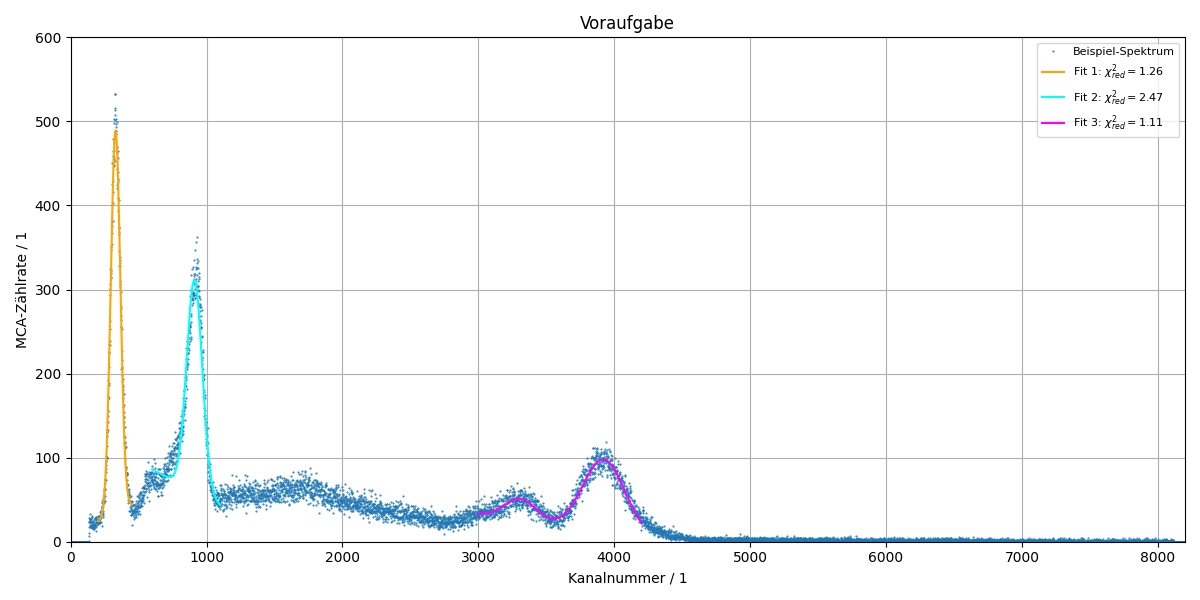
\includegraphics[width=\textwidth]{figs/voraufgabe_fertig.png}
    \caption{Beispielspektrum mit den durch das Auswerteprogramm angepassten Gaußfunktionen. 
    In der Legende sind zusätzlich die jeweiligen Werte des reduzierten Chi-Quadrats $\chi^2_\mathrm{red}$ angegeben.}
    \label{fig:voraufgabe_fit}
\end{figure}
